\section{URDAD in the context of Model-Driven Development}
\label{sec:contextualization}

In model-driven development (MDD) \cite{stahl:mdsd, france:mddUsingUml2},
and the Object Management Group's (OMG) Model Driven Architecture
(MDA) \cite{stahl:mdsd, france:mddUsingUml2} in particular,
the core artifact is the model which specified in terms of concepts
from the problem domain instead of the solution domain.
The model thus needs to be generated and maintained by domain
experts (e.g.\ business analysts in the context of enterprise systems development)
and not by technical specialists.

The model contains the functional requirements, together with the processes 
and other design elements (such as the data structures required by the processes) through which the functional requirements are realized.

The information about the technical infrastructure within which the model needs to
be implemented is provided by a separate architecture/technologies specification, which can vary
independently from the functional model. The architecture needs to be designed such that the infrastructure
is able to address the non-functional requirements of the services (e.g.\ performance, scalability, reliability,
security, auditability, accessibility, usability, ...). In the context of enterprise architecture,
the architecture spans across organizational and systems architecture, providing the organization with a suitable infrastructure within which it can realize its vision and mission, and within which business processes
are deployed and executed. It seamlessly encompasses software, hardware and human components.

\begin{figure}[!t]
  \centering
	\includegraphics[width=2.5in]{mdaProcess}	
  \caption{Separation of functionality and architecture/technologies as envisaged by the MDA.}
  \label{fig:mda}
\end{figure}

Figure \ref{fig:mda} shows MDA's envisaged separation of architecture/technology from process design. Once the process addressing the functional requirements has been designed, the
implementation mapping of the resultant platform independent model (PIM) into the architecture designed to address the quality requirements can be automated using MDA tools. The tools can also potentially be used to perform other transformations like that of transforming the URDAD model into a formal methods-based representation, like a Petri Net or documentation generation.

One of the aims of model-driven development is the clean separation of responsibilities across
architecture, (business) analysis, implementation mapping, quality assurance and operations. A typical model driven development process is shown in figure \ref{fig:developmentProcess}.

\begin{figure}[!t]
  	\centering
	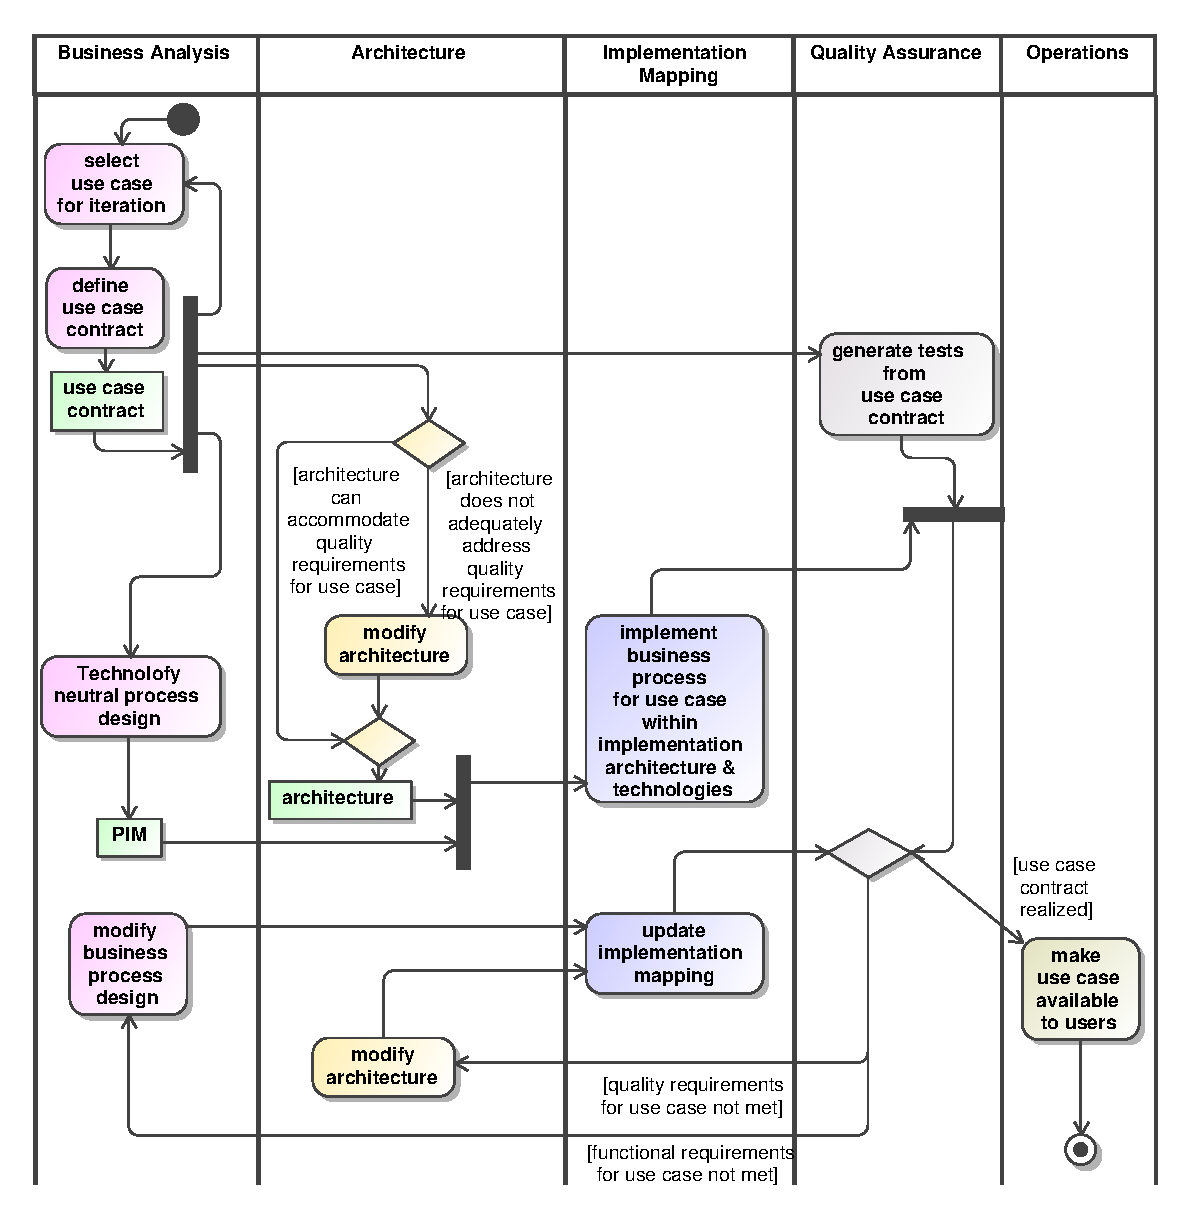
\includegraphics[width=2.5in]{developmentProcess}
  	\caption{Separation of concerns in a typical model-driven developmen process.}
  	\label{fig:developmentProcess}
\end{figure}

The domain/business analysts perform the stake holder requirements elicitation, validation and documentation resulting in a use case or services contract. This contract is used by quality
assurance (QA) to (auto)-generate the functional and non-functional tests. Architecture assesses whether the current infrastructure can host the service with its particular quality requirements and, if required, makes the necessary architectural modifications. Domain analysts then perform the technology neutral process design. It is for this step that URDAD is used. Once the technology neutral design is complete and once architecture has signed off the architecture specification, the implementation mapping is done after which QA will have to assess whether both, the functional and non-functional requirements are fulfilled. In the case where there are issues with the functional requirements (i.e.\ with what has or has not been done), the error reports are provided to domain analysis which then either makes the required modifications to the technology neutral design or notifies implementation mapping that certain mappings have been implemented incorrectly. In either case the implementation mapping is updated after which it goes back to QA.

On the other hand, should QA finds quality of service issues (e.g.\ performance, security, reliability, scalability, ..., issues), the problem is reported to architecture which either makes appropriate architectural modifications or notifies implementation mapping of concerns with the implementation. Once QA has verified the realization of the use case contract, the service is handed over to operations to be made available to the users.